\documentclass{beamer}

%% \documentclass[handout]{beamer}
%% % use this with the [handout] option to create handouts for the audience
%% \usepackage{pgfpages}
%% \pgfpagesuselayout{2 on 1}[a4paper,border shrink=5mm]

\mode<presentation>
{
  \usetheme{Diku}
% set this to your preferences:
  \setbeamercovered{invisible}
%  \setbeamercovered{transparent}
}

\usepackage{graphicx}
\usepackage{epic}

\usepackage{amsmath}
\usepackage{amssymb}
\usepackage{amsthm}

\newcommand{\basetop}[1]{\vtop{\vskip-1ex\hbox{#1}}}
\newcommand{\source}[1]{\let\thefootnote\relax\footnotetext{\scriptsize\textcolor{kugray1}{Source: #1}}}

% for coloured code citation in text:
\usepackage{fancyvrb}

%%%%%%%%%%%%%%%%%%%%%%%%%%%%%%%%%
%%%%%    code sections   %%%%%%%%
%%%%%%%%%%%%%%%%%%%%%%%%%%%%%%%%%

% code highlighting commands in own block
\DefineVerbatimEnvironment{code}{Verbatim}{fontsize=\scriptsize}
\DefineVerbatimEnvironment{icode}{Verbatim}{fontsize=\scriptsize}

% Fancy code with color commands:
\DefineVerbatimEnvironment{colorcode}%
        {Verbatim}{fontsize=\scriptsize,commandchars=\\\{\}}

%%%%%%%%%%%%%%%%%%%%%%%%%%%%%%%%%%
%%%%%    some coloring    %%%%%%%%

\definecolor{Red}{RGB}{220,50,10}
\definecolor{Blue}{RGB}{0,51,102}
\definecolor{Yellow}{RGB}{102,51,0}
\definecolor{Orange}{RGB}{178,36,36}
\definecolor{Grey}{RGB}{180,180,180}
\definecolor{Green}{RGB}{20,120,20}
\definecolor{Purple}{RGB}{160,50,100}
\newcommand{\red}[1]{\textcolor{Red}{{#1}}}
\newcommand{\blue}[1]{\textcolor{Blue}{{#1}}}
\newcommand{\yellow}[1]{\textcolor{Yellow}{{#1}}}
\newcommand{\orange}[1]{\textcolor{Orange}{{#1}}}
\newcommand{\grey}[1]{\textcolor{Grey}{{#1}}}
\newcommand{\green}[1]{\textcolor{Green}{{#1}}}
\newcommand{\purple}[1]{\textcolor{Purple}{{#1}}}




% use "DIKU green" from our color theme for \emph
\renewcommand{\emph}[1]{\textcolor{structure}{#1}}
% use some not-too-bright red for an \emp command
\definecolor{DikuRed}{RGB}{130,50,32}
\newcommand{\emp}[1]{\textcolor{DikuRed}{ #1}}
\definecolor{CosGreen}{RGB}{10,100,70}
\newcommand{\emphh}[1]{\textcolor{CosGreen}{ #1}}
\definecolor{CosBlue}{RGB}{55,111,122}
\newcommand{\emphb}[1]{\textcolor{CosBlue}{ #1}}
\definecolor{CosRed}{RGB}{253,1,1}
\newcommand{\empr}[1]{\textcolor{CosRed}{ #1}}

\newcommand{\mymath}[1]{$ #1 $}
\newcommand{\myindx}[1]{_{#1}}
\newcommand{\myindu}[1]{^{#1}}

\newcommand{\Fasto}{\textsc{Fasto}\xspace}


%%%%%%%%%%%%%%%%%%%%

\title[Machine Code]{Machine Code Generation}

\author[C.~Oancea]{Cosmin E. Oancea\\{\tt cosmin.oancea@diku.dk}}

\institute{Department of Computer Science (DIKU)\\University of Copenhagen}


\date[December 2012]{December 2012 Compiler Lecture Notes}


\begin{document}

\titleslide

\begin{frame}
\frametitle{Structure of a Compiler}

\begin{tabular}{ccc}
Program text&&\\
$\downarrow$ &&\\
\framebox{Lexical analysis} && Binary machine code\\
$\downarrow$ && $\uparrow$ \\
Symbol sequence && \textcolor{gray}{\framebox{Assembly and linking}} \\
$\downarrow$ && $\uparrow$ \\
\framebox{Syntax analysis} && Ditto with named registers\\
$\downarrow$ && $\uparrow$ \\
Syntax tree && \framebox{Register allocation} \\
$\downarrow$ && $\uparrow$ \\
\framebox{Type Checking} && Symbolic machine code\\
$\downarrow$ &&  $\uparrow$ \\
Syntax tree  && \framebox{\red{Machine code generation}} \\
$\downarrow$ && $\uparrow$ \\
\framebox{Intermediate code generation} &$\longrightarrow$ & Intermediate code
\end{tabular}

\end{frame}


\begin{frame}[fragile]
	\tableofcontents
\end{frame}


%%%%%%%%%%%%%%%%%%%%%%%%%%%%%%%%%%%%%%%%%%%%%%%%%%%%%%%%%%%%%%%%%%%%%%
%%%%%%%%%%%%%%%%%%%%%%%%%%%%%%%%%%%%%%%%%%%%%%%%%%%%%%%%%%%%%%%%%%%%%%
\section{Quick Look at MIPS}

\begin{frame}[fragile,t]
   \frametitle{Symbolic Machine Language}

\bigskip
\bigskip

A text-based representation of binary code:

\bigskip

\begin{itemize}

    \item more readable than machine code,\bigskip

    \item uses labels as destinations of jumps,\bigskip

    \item allows constants as operands,\bigskip

    \item translated to binary code by {\em assembler} and {\em linker}.

\end{itemize}

\end{frame}


\begin{frame}[fragile,t]
   \frametitle{Remember MIPS?}

\begin{description}

    \item[.data:] the upcoming section is considered data,\smallskip

    \item[.text:] the upcoming section consists of instructions,\smallskip

    \item[.global:] the label following it is accessible from outside,\smallskip

    \item[.asciiz "Hello":]  string with null terminator,\smallskip

    \item[.space n:] reserves n bytes of memory space,\smallskip

    \item[.word w1, .., wn:] reserves n words.
\end{description}


\begin{block}{Mips Code Example: \$ra = \$31, \$sp = \$29, \$hp = \$28 (heap pointer)}
\begin{columns}
\column{0.44\textwidth}\vspace{-2ex}
\begin{colorcode}[fontsize=\scriptsize]
        .data
val:    .word 10, -14, 30
str:    .asciiz "Hello!"
_heap_: .space 100000
        .text
        .global main
        la \$28, _heap_
        jal main
        ...
\end{colorcode} 
\column{0.44\textwidth}\vspace{-2ex}
\begin{colorcode}[fontsize=\scriptsize]
_stop_:
         ori  \$2, \$0, 10
         syscall
main:
         la   \$8, val    # ?
         lw   \$9, 4(\$8)  # ?
         addi \$9, \$9, 4  # ?
         sw   \$9, 8(\$8)  #...
         j    _stop_     #jr \$31
\end{colorcode}
\end{columns}
\end{block}

\pause
\smallskip

The third element of val, i.e., $30$, is set to $-14 + 4 = -10$.

\end{frame}

%%%%%%%%%%%%%%%%%%%%%%%%%%%%%%%%%%%%%%%%%%%%%%%%%%%%%%%%%%%%%%%%%%%%%%
%%%%%%%%%%%%%%%%%%%%%%%%%%%%%%%%%%%%%%%%%%%%%%%%%%%%%%%%%%%%%%%%%%%%%%
\section{Intermediate {\em vs} Machine Code}

\begin{frame}[fragile]
	\tableofcontents[currentsection]
\end{frame}

\begin{frame}[fragile,t]
   \frametitle{Intermediate and Machine Code Differences}

\bigskip
\bigskip

\begin{itemize}

    \item \alert{machine code has a limited number of registers,}\bigskip

    \item \alert{usually there is no equivalent to \texttt{CALL}, i.e., need to implement it,}\bigskip

    \item conditional jumps usually have only one destination,\bigskip

    \item comparisons may be separated from the jumps,\bigskip

    \item typically {\sc risc} instructions allow only small-constant operands.

\end{itemize}

\bigskip
\bigskip

\alert{The first two issues are solved in the next two lessons.}


\end{frame}


\begin{frame}
\frametitle{Two-Way Conditional Jumps}

${\tt IF}~c~{\tt THEN}~l_t~{\tt ELSE}~l_f$ can be translated to:

\begin{tabular}{ll}\\
\emp{{\tt~~~~branch\underline{~}if\underline{~}cond}} & \emp{$l_t$} \\
\emp{{\tt~~~~jump}} & \emp{$l_f$}\\
\\
\end{tabular}

\bigskip

If $l_t$ or $l_f$ follow right after {\sc if-then-else}, we can \emph{eliminate one jump}:\smallskip

\emp{\tt~~~~~IF c THEN $l_t$ ELSE $l_f$}\\
\emp{\tt{}$l_t$:}\\
\emp{\tt~~~~~...}\\
\emp{\tt{}$l_f$:}

\smallskip

can be translated to:\smallskip

\emp{\tt~~~~~branch\_if\_not\_cond $l_f$}

\end{frame}



\begin{frame}[fragile,t]
   \frametitle{Comparisons}

\bigskip

In many architectures the comparisons are separated from the jumps:
\emp{first evaluate the comparison, and place the result in a register that
can be later read by a jump instruction.}


\bigskip

\begin{itemize}

    \item In \textsc{mips} both $=$ and $\not=$ operators can jump ({\tt beq} and {\tt bne}),\\ 
        but $<$ ({\tt slt}) stores the result in a general register.\bigskip

    \item \textsc{arm} and {\tt X86}'s arithmetic instructions set a \emp{flag} 
            to signal that the result is $0$ or negative, or overflow, or carry, etc.\bigskip

    \item {\tt PowerPC} and {\tt Itanium} have \emp{separate boolean registers}.\bigskip

\end{itemize}

\end{frame}


\begin{frame}[fragile,t]
   \frametitle{Constants}

\bigskip

Typically, machine instructions restrict \emp{\em constants' size} to be 
\blue{smaller than one machine word}:\smallskip

\begin{itemize}

    \item {\sc mips32} uses $16$ bit constants. For \emp{\em larger constants}, \blue{\tt lui} 
        is used to load a $16$-bit constant into \blue{the upper half of a $32$-bit register}.\smallskip

    \item {\sc arm} allows $8$-bit constants, which can be positioned at any 
            (even-bit) position of a $32$-bit word.

\end{itemize}


\bigskip

\emp{Code generator checks if the constant value fits the restricted size:}

\begin{description}

    \item[{\em if it fits:}] it generates one machine instruction (constant operand);\smallskip

    \item[{\em otherwise:}] use an instruction that uses a register (instead of a ct)
            generate a sequence of instructions that load the
            constant value in that register.

\end{description}

\bigskip

\emp{Sometimes, the same is true for the jump label.}

\end{frame}


\begin{frame}[fragile,t]
    \frametitle{Demonstrating Constants}

\begin{block}{\textsc{Fasto} Implementation}
\begin{colorcode}[fontsize=\scriptsize]
fun compileExp e vtable place =
    case e of
      Fasto.Num (n,pos)   =>
        if ( \emph{n < 65536} )
        then [ \emph{Mips.LI (place, makeConst n)}                    ]
        else [ \emp{Mips.LUI (place, makeConst(n div 65536)),}
               \emp{Mips.ORI (place, place, makeConst(n mod 65536))} ]
\end{colorcode} 
\end{block}

\bigskip

\emp{What happens with negative constants?}

\end{frame}

%%%%%%%%%%%%%%%%%%%%%%%%%%%%%%%%%%%%%%%%%%%%%%%%%%%%%%%%%%%%%%%%%%%%%%
%%%%%%%%%%%%%%%%%%%%%%%%%%%%%%%%%%%%%%%%%%%%%%%%%%%%%%%%%%%%%%%%%%%%%%
\section{Exploiting Complex Instructions}

\begin{frame}[fragile]
	\tableofcontents[currentsection]
\end{frame}


\begin{frame}[fragile,t]
   \frametitle{Exploiting Complex Instructions}

\bigskip


Many architectures expose complex instructions that combine several
operations (into one), e.g.,\smallskip

\begin{itemize}

    \item load/store instruction also involve address calculation,\bigskip

    \item arithmetic instructions that scales one argument (by shifting),\bigskip

    \item saving/restoring multiple registers to/from memory storage,\bigskip

    \item conditional instructions (other besides jump).

\end{itemize}

\bigskip

In some cases: several {\sc il} instructions $\rightarrow$ one machine instruction.\\\smallskip
In other cases: one {\sc il} instruction $\rightarrow$ several machine instructions,
e.g., conditional jumps.

\end{frame}



\begin{frame}[fragile,t]
   \frametitle{MIPS Example}

\bigskip

The two intermediate-code instructions:
\smallskip

\emp{\tt~~~~~~~~~~t2 := t1 + 116}\\
\emp{\tt~~~~~~~~~~t3 := M[ t2 ]}

\bigskip

can be combined into {\em one} {\sc mips} instruction (?)
\smallskip

\emph{\tt~~~~~~~~~~lw r3, 116(r1)}

\bigskip

\emph{{\sc iff} $t_2$ is not used anymore}! Assume that we mark/know whenever a 
        variable is used for the last time in the intermediate code.
\bigskip

This marking is accomplished by means of \blue{\em liveness analysis}; we write:
\smallskip

\emp{\tt~~~~~~~~~~t2 := t1 + 116}\\
\emp{\tt~~~~~~~~~~t3 := M[ t2$^{last}$ ]}

\end{frame}



\begin{frame}[fragile,t]
   \frametitle{Intermediate-Code Patterns}

\bigskip

\begin{itemize}

    \item Need to map \emph{each {\sc il} instruct} to one or many machine instructs.\smallskip

    \item Take advantage of complex-machine instructions via \emp{\em patterns}:
            \begin{itemize}
                \item map \emp{a sequence of {\sc il} instructs} to one or many machine instructs,
                \item try to match first the longer pattern, i.e., the most profitable one.\smallskip
            \end{itemize}

    \item Variables marked with {\em last} in the {\sc il} pattern {\em must} be matched
            with variables that are used for the last time in the il code.\smallskip

    \item The converse is not necessary:

\end{itemize}

\[ \begin{array}{|l|l|}\hline
t := r_s + k & \mbox{\tt lw}~r_t,\,k(r_s) \\
r_t := M[t^{last}] &\\\hline
\end{array}\]

\smallskip

$t$, $r_s$ and $r_t$ can match arbitrary {\sc il} variables, $k$ can match any constant 
(big constants have already been eliminated).

\end{frame}


\begin{frame}
\frametitle{Patterns for MIPS (part 1)}

\renewcommand{\arraystretch}{0.9}
\begin{tabular}{|l|lll|}\hline

$ t := r_s + k,$
&&  {\tt lw} & $r_t,~k(r_s)$ \\
$r_t := M[t^{last}]$ &&& \\\hline

$ r_t := M[r_s]$
&&  {\tt lw} & $r_t,~0(r_s)$ \\\hline

$ r_t := M[k]$
&&  {\tt lw} & $r_t,~k$({\tt R0}) \\\hline

$ t := r_s + k,$
&&  {\tt sw} & $r_t,~k(r_s)$ \\
$M[t^{last}] := r_t$ &&&  \\\hline

$ M[r_s] := r_t$
&&  {\tt sw} & $r_t,~0(r_s)$ \\\hline

$ M[k] := r_t$
&&  {\tt sw} & $r_t,~k$({\tt R0}) \\\hline

$  r_d := r_s + r_t  $
&&  {\tt add} & $r_d$, $r_s$, $r_t$ \\\hline

$  r_d := r_t  $
&&  {\tt add} & $r_d$, {\tt R0}, $r_t$ \\\hline

$  r_d := r_s + k  $
&&  {\tt addi} & $r_d$, $r_s$, $k$ \\\hline

$  r_d := k  $
&& {\tt addi} & $r_d$, {\tt R0}, $k$ \\\hline

$  {\tt GOTO}~label  $ 
&& {\tt j} & $label$ \\\hline

\end{tabular}

\bigskip

Must cover all possible sequences of intermediate-code instructions.

\end{frame}



\begin{frame}
\frametitle{Patterns for MIPS (part 2)}

\renewcommand{\arraystretch}{0.9}
\begin{tabular}{|l|lll|}\hline


$  {\tt IF}~r_s = r_t~{\tt THEN}~label_t~ {\tt ELSE}~ label_f,$
&&  {\tt beq} & $r_s$, $r_t$, $label_t$ \\
{\tt LABEL}~$label_f  $
& $label_f$: & & \\\hline

$  {\tt IF}~r_s = r_t~{\tt THEN}~label_t~ {\tt ELSE}~ label_f,$
&&  {\tt bne} & $r_s$, $r_t$, $label_f$ \\
{\tt LABEL}~$label_t  $
& $label_t$: & & \\\hline

$  {\tt IF}~r_s = r_t~{\tt THEN}~label_t~ {\tt ELSE}~ label_f $
&& {\tt beq} & $r_s$, $r_t$, $label_t$ \\
&& {\tt j} & $label_f$ \\\hline

$  {\tt IF}~r_s < r_t~{\tt THEN}~label_t~ {\tt ELSE}~ label_f,$
&&  {\tt slt} & $r_d$, $r_s$, $r_t$ \\
{\tt LABEL}~$label_f  $
&&  {\tt bne} & $r_d$,~{\tt R0},~ $label_t$ \\
& $label_f$: & & \\\hline

$  {\tt IF}~r_s < r_t~{\tt THEN}~label_t~ {\tt ELSE}~ label_f,$
&& {\tt slt} & $r_d$, $r_s$, $r_t$ \\
{\tt LABEL}~$label_t  $
&&  {\tt beq} & $r_d$,~{\tt R0},~ $label_f$\\
& $label_t$: & & \\\hline

$  {\tt IF}~r_s < r_t~{\tt THEN}~label_t~ {\tt ELSE}~ label_f  $ 
&&  {\tt slt} & $r_d$, $r_s$, $r_t$ \\
&& {\tt bne} & $r_d$,~{\tt R0},~$label_t$ \\
&&  {\tt j} & $label_f$ \\\hline

{\tt LABEL}~$label$ & $label$: && \\\hline

\end{tabular}

\end{frame}




\begin{frame}
\frametitle{Compiling Code Sequences: Example}

\bigskip
\bigskip

\renewcommand{\arraystretch}{0.9}
\[\begin{array}{l}
a := a+b^{last} \\
d := c+8 \\
M[d^{last}] := a \\
{\tt IF}~a = c~{\tt THEN}~label_1~ {\tt ELSE}~ label_2 \\
{\tt LABEL}~label_2
\end{array}\]

\end{frame}


\begin{frame}
\frametitle{Compiling Code Sequences}

Example:
\renewcommand{\arraystretch}{0.9}
\[\begin{array}{l|lll}
a := a+b^{last} & & {\tt add} & a,~a,~b \\
d := c+8 & & {\tt sw} & a,~8(c) \\
M[d^{last}] := a & && \\
{\tt IF}~a = c~{\tt THEN}~label_1~ {\tt ELSE}~ label_2 &
 & {\tt beq} & a,~c,~label_1 \\
{\tt LABEL}~label_2~& label_2:&&
\end{array}\]

\bigskip
Two approaches:
\smallskip

\begin{description}

\item[Greedy Alg:] Find the first/longest pattern matching a prefix of the
                    {\sc il} code $+$ translate it. Repeat on the rest of the code.\smallskip


\item[Dynamic Prg:] Assign to each machine instruction a cost and find the
                        matching that minimize the global / total cost.

\end{description}

\end{frame}




\begin{frame}
\frametitle{Two-Address Instructions}

Some processors, e.g., {\tt X86}, store the instruction's result in one of the
operand registers. Handled by placing one argument in the result register and 
then carrying out the operation:

\bigskip

\renewcommand{\arraystretch}{0.9}
\begin{center}
\begin{tabular}{|l|lll|}\hline

$ r_t := r_s $
&&  {\tt mov} & $r_t,~r_s$ \\\hline

$ r_t := r_t+r_s$
&& {\tt add} & $r_t,r_s$ \\\hline

$  r_d := r_s + r_t  $
&&  {\tt move} & $r_d$, $r_s$ \\
&&  {\tt add} & $r_d,r_t$ \\\hline
\end{tabular}
\end{center}

\bigskip

Register allocation can remove the extra {\tt move}.

%Division into data and address registers or integer and FP registers can
%handled in the same way.

\end{frame}



\begin{frame}
\frametitle{Optimizations}

Can be performed at different levels:\smallskip

\begin{description}
\item[Abstract Syntax Tree:] high-level optimization: specialization, 
                inlining, map-reduce, etc.\smallskip


\item[Intermediate Code:] machine-independent optimizations, such as
                redundancy elimination, or index-out-of-bounds checks.\smallskip

\item[Machine Code:] machine-specific, low-level optimizations such as
                        instruction scheduling and pre-fetching.

\end{description}

\bigskip

Optimizations at the intermediate-code level can be shared between
different languages and architectures.

\bigskip

\vspace{1ex}

We talk more about optimizations next lecture and in the New Year!

\end{frame}


%%%%%%%%%%%%%%%%%%%%%%%%%%%%%%%%%%%%%%%%%%%%%%%%%%%%%%%%%%%%%%%%%%%%%%
%%%%%%%%%%%%%%%%%%%%%%%%%%%%%%%%%%%%%%%%%%%%%%%%%%%%%%%%%%%%%%%%%%%%%%
\section{Machine-Code Generation in \textsc{Fasto}}

\begin{frame}[fragile]
	\tableofcontents[currentsection]
\end{frame}



\begin{frame}[fragile,t]
   \frametitle{\textsc{Fasto} Arrays}

\bigskip

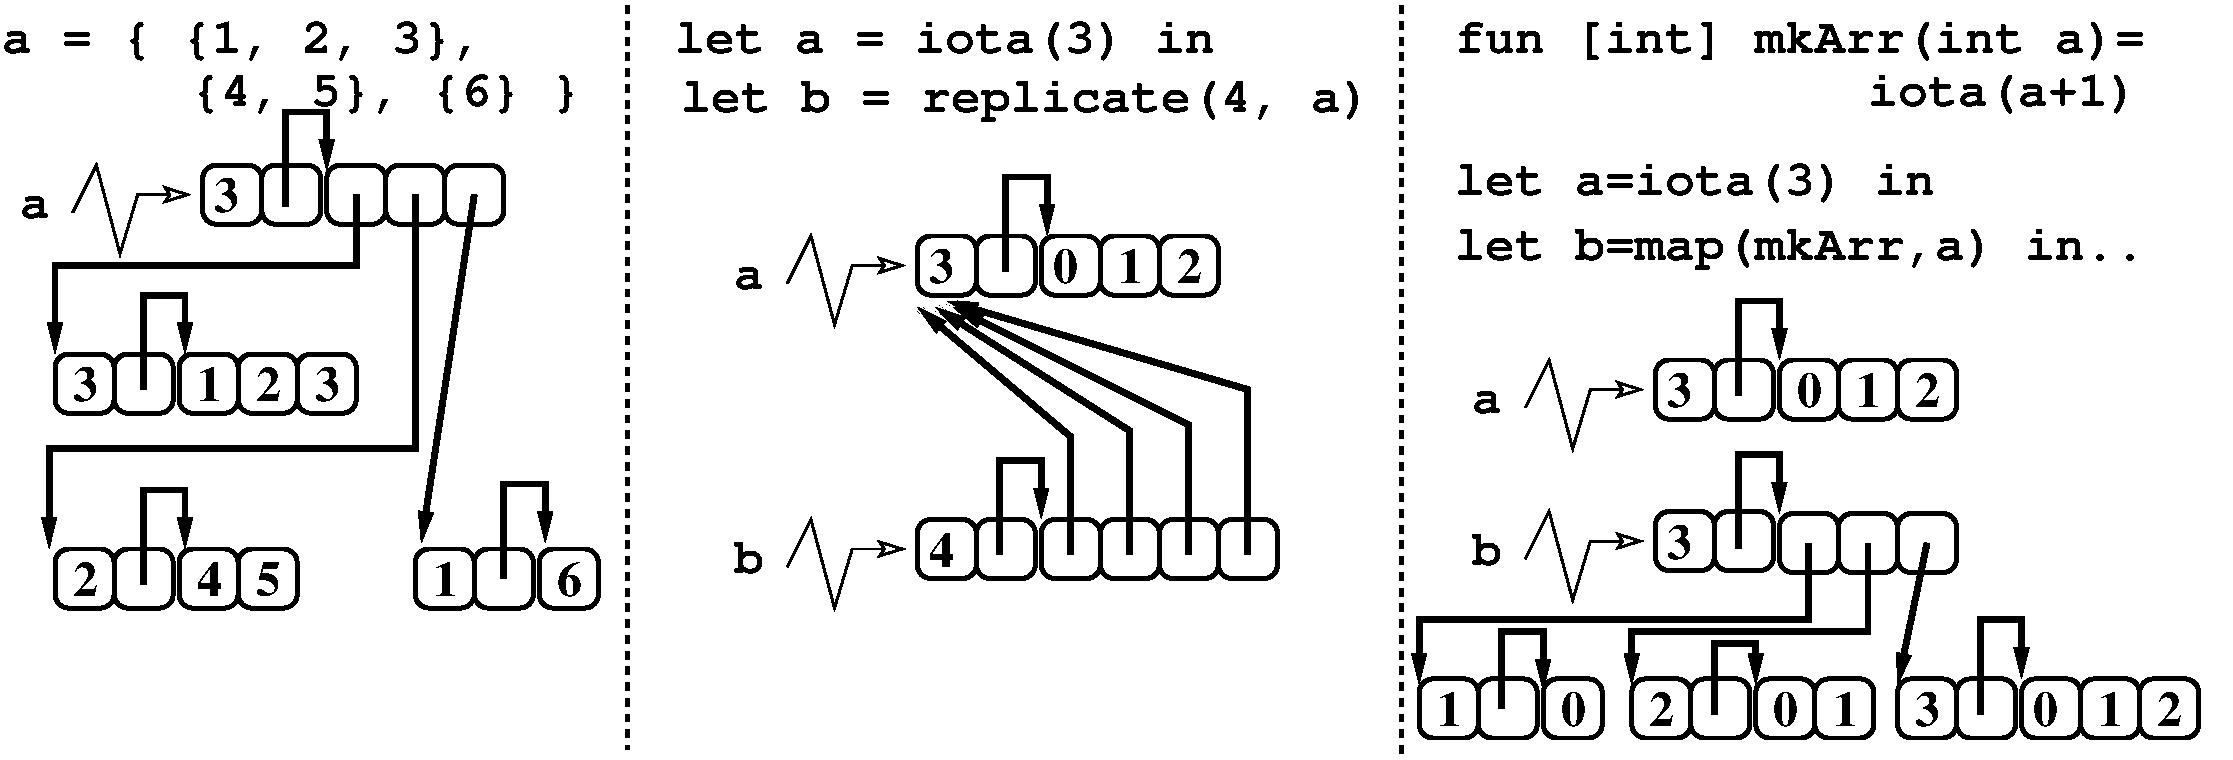
\includegraphics[width=70ex]{Figures/ArraysPrecise}

\bigskip

Let us translate \emp{\tt let a2 = map(f, a1)}, where \emp{\tt a1,a2~:~[int]}
and \emph{$R_{a1}$} holds \emp{\tt a1}, \emph{$R_{a2}$} holds \emp{\tt a2}, 
\emph{$R_{HP}$} is the heap pointer.

\end{frame}


\begin{frame}[fragile,t]
    \frametitle{Example: Translation of {\tt let a2 = map(f, a1)}}

\begin{block}{$R_{a1}$ holds {\tt a1}, $R_{a2}$ holds {\tt a2}, 
$R_{HP}$ is the heap pointer, {\tt a1,a2~:~[int]}}
\begin{columns}
\column{0.29\textwidth}
\begin{colorcode}[fontsize=\scriptsize]
\green{len = length(a1)}
\blue{a2  = malloc(len*4)}
\emp{i = 0}
\emp{while(i < len) \{}
    tmp   = f(a1[i]);
    a2[i] = tmp;
\emp{\}}
\end{colorcode}
 
\column{0.24\textwidth}
\begin{colorcode}[fontsize=\scriptsize]
\green{lw   \mymath{R\myindx{len}} , 0(\mymath{R\myindx{a1}})}
\blue{move \mymath{R\myindx{a2}} , \mymath{R\myindx{HP}}}
\blue{sll  \mymath{R\myindx{tmp}}, \mymath{R\myindx{len}}, 2}
\blue{addi \mymath{R\myindx{tmp}}, \mymath{R\myindx{tmp}}, 8}
\blue{add  \mymath{R\myindx{HP}}, \mymath{R\myindx{HP}}, \mymath{R\myindx{tmp}}}
\blue{sw   \mymath{R\myindx{len}} , 0(\mymath{R\myindx{a2}})}
\blue{addi \mymath{R\myindx{tmp}}, \mymath{R\myindx{a2}} , 8}
\blue{sw   \mymath{R\myindx{tmp}}, 4(\mymath{R\myindx{a2}})}
\emp{lw   \mymath{R\myindx{it1}} , 4(\mymath{R\myindx{a1}})}
\emp{lw   \mymath{R\myindx{it2}} , 4(\mymath{R\myindx{a2}})}
\emp{move \mymath{R\myindx{i}}  , \$0}
\end{colorcode}

\column{0.37\textwidth}
\begin{colorcode}[fontsize=\scriptsize]
\emp{loop\mymath{\myindx{beg}}:}
\emp{        sub    \mymath{R\myindx{tmp}}, \mymath{R\myindx{i}}, \mymath{R\myindx{len}}}
\emp{        bgez   \mymath{R\myindx{tmp}}, loop\mymath{\myindx{end}}}
        lw     \mymath{R\myindx{tmp}}, 0(\mymath{R\myindx{it1}})
        addi   \mymath{R\myindx{it1}}, \mymath{R\myindx{it1}}, 4
\alert{        \mymath{R\myindx{tmp}} = CALL f(\mymath{R\myindx{tmp}})}
        sw     \mymath{R\myindx{tmp}}, 0(\mymath{R\myindx{it2}})
        addi   \mymath{R\myindx{it2}}, \mymath{R\myindx{it2}}, 4
        addi   \mymath{R\myindx{i}}, \mymath{R\myindx{i}}, 1
\emp{        j      loop\mymath{\myindx{beg}}}
\emp{loop\mymath{\myindx{end}}:}
\end{colorcode}
\end{columns}
\end{block}

\bigskip
Compiler.sml:\smallskip
\begin{description}

    \item[dynalloc] generates code to allocate an array,\smallskip

    \item[ApplyRegs] generates code to call a function on a list of arguments (registers).\smallskip

\end{description}

\end{frame}

%%%%%%%%%%%%%%%%%%%%%%%%%%%%%%%%%%%%%%%%%%%%%%%%%%%%%%%%%%%%%%%%%%%%%%
%%%%%%%%%%%%%%%%%%%%%%%%%%%%%%%%%%%%%%%%%%%%%%%%%%%%%%%%%%%%%%%%%%%%%%





\end{document}
